\documentclass{udpreport}
\title{Creación de paquetes utilizando Scapy y validación con Wireshark}
\author{Integrantes: Thomas Muñoz, Ignacio Yanjari, Dagoberto Navarrete, Ignacio López.}
\date{Marzo de 2016}
\usepackage{graphicx}
\graphicspath{ {img/} }
\udpschool{Escuela de Informática y Telecomunicaciones}

\begin{document}
\maketitle
\tableofcontents
\chapter{Introducción}
	En este laboratorio buscamos aprender cómo se crean los paquetes con Scapy y como se organizan estos, además de entender la
	diferencia entre enviar un paquete a un equipo específico o a todos los pertenecientes a la red, a su vez entendimos la
	utilidad de Wireshark al tener que filtrar y capturar los paquetes que enviábamos entre nuestros equipos para verificar que se
	hayan recibido correctamente y estos no tuvieran algún tipo de problema.
\chapter{Actividades}
	\section{Instalacion de software}

	\section{Creacion de Paquetes}
		Para la creación de paquetes fue necesario aplicar nuestros conocimientos sobre la composición de un frame.
		Los frames cuentan con un Preámbulo el cual lleva una secuencia específica de bits para que el receptor note si el
		frame llega en buen estado o no, cuenta con un Delimitador de inicio el cual avisa al receptor que luego de una
		secuencia definida de unos y ceros se dará inicio a la información del frame, también cuenta con la dirección de
		destino y origen (MAC e IP), más adelante vienen unos bits donde se le da a conocer al receptor el largo de los datos
		del frame, para luego continuar con el Encabezado y datos reales del frame (mensaje) y para finalizar la trama hay una
		Secuencia de verificación donde se vuelve a verificar que esta esté sin errores.\\
		
		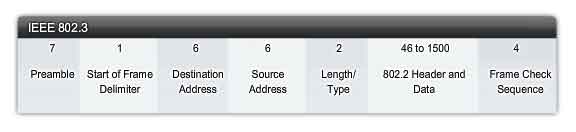
\includegraphics[width=\textwidth]{frame.jpg}\\
		(frame según el estandar IEEE 802.3)
		Estos paquetes se e
	\section{Cuestionario}
	
	  1.-¿Qué pasa cuando envío un paquete a la dirección FF:FF:FF:FF:FF:FF? ¿Quienes
	     lo reciben? ¿Por qué?\\
    			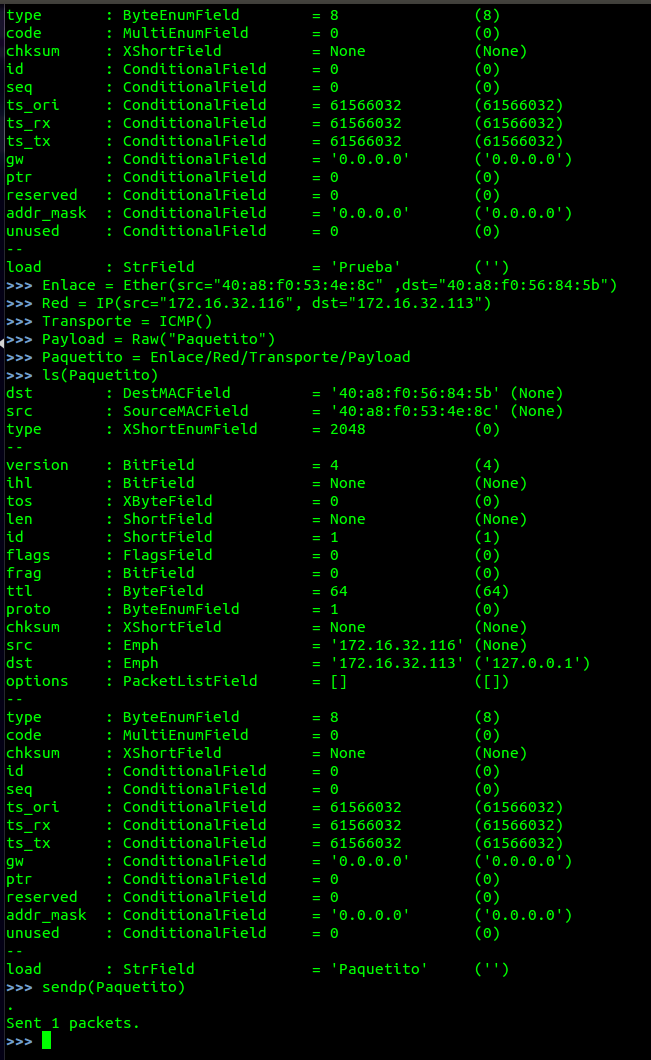
\includegraphics[width=4cm, height=4.3cm]{EnvioPaquetito.png}  
	     Cuando enviamos un paquete a la dirección FF:FF:FF:FF:FF:FF, este fue enviado a todos los equipos dentro de la red
	     Ethernet. Esto es debido a que la dirección antes mencionada esta designada para que la difusión de nuestro paquete sea
 	     enviado a cada dispositivo conectado a nuestra red LAN, a este tipo de difusión se le conoce como “Broadcast”.\\
 
  	  2.-¿Qué pasa cuando envío un paquete a una MAC de otro equipo? ¿Quienes lo
  	      pueden recibir? ¿Por qué?\\
    			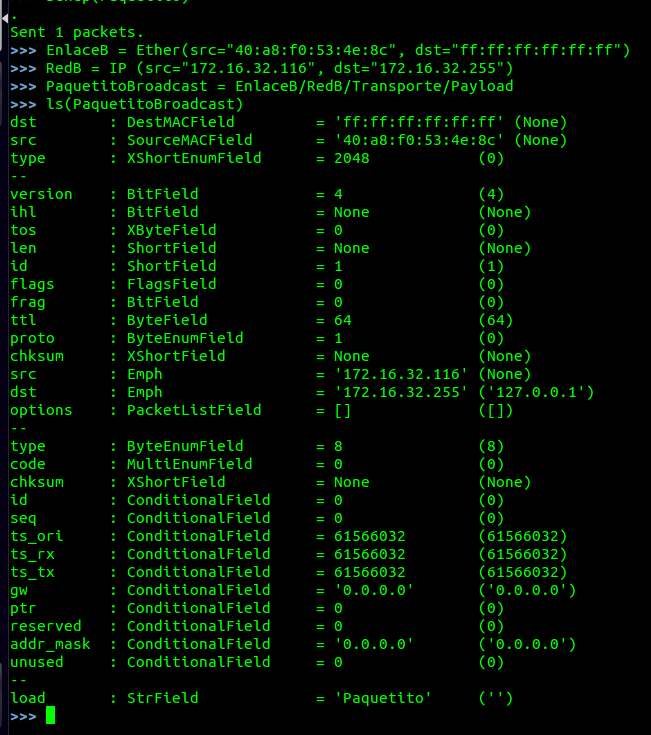
\includegraphics[width=4cm, height=4.3cm]{EnvioPaquetitoMalo2.png}
 	      
 	      Cuando enviamos un paquete a la dirección MAC de otro equipo dentro de la red Ethernet, solamente el equipo que poseía
 	      esa dirección fue capaz de recibirlo. Esto ocurre puesto a que, como indicamos anteriormente, al paquete le dimos una
 	      MAC de destino fija, entonces el paquete se encargó de viajar solamente al equipo que poseía esa dirección\\
 
  	  3.-¿Qué sucede si envía un paquete a una MAC que no corresponda a ningún equipo
  	      de la red? ¿Quienes lo pueden recepcionar? ¿Por qué?\\
    			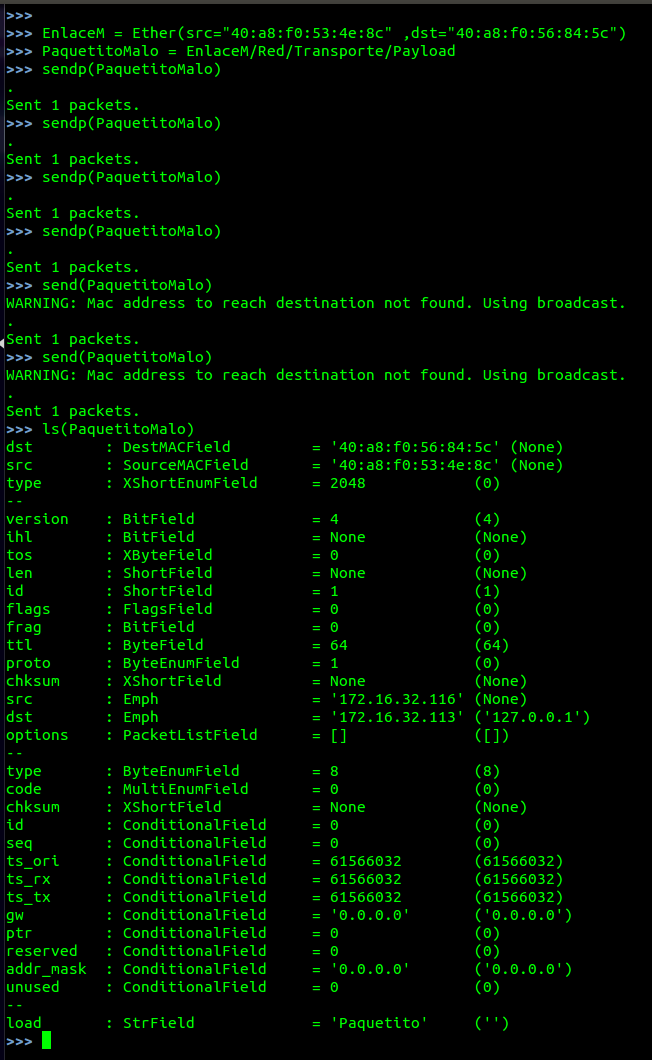
\includegraphics[width=4cm, height=4.3cm]{EnvioPaquetitoMalo.png}
 	      Cuando enviamos un paquete a una dirección MAC que no correspondía a ningún equipo de la red, al enviarlo nos apareció
 	      el mensaje: “WARNING: Mac address to reach destination not found. Using Broadcast.” Y posteriormente el paquete fue
 	      enviado a todos los equipos pertenecientes a la red Ethernet. Se usa el Broadcast para así poder obtener todas las
 	      direcciónes MAC mediante su IP, registrarlas en la lista arp y encontrar la que se dio como destinataria, pero como esta
 	      no se encuentra en la red sigue mandando el paquete a todos los equipos que si están en la red para seguir buscando la
 	      MAC solicitada.\\

 	     
	      

\chapter{Conclusión}
  	      En esta experiencia de laboratorio se logra comprender cómo crear correctamente un paquete con Scapy,
  	      entendiendo todos sus componentes y cómo se puede enviar al o a los destinatarios que nosotros deseemos, también
  	      logra dejar clara la diferencia entre los comandos “send()” y “sendp()”, la capa en la que trabajan y cuando usar cada
  	      uno,se capta la forma en como funciona un Switch y un Hub con respecto al envío de paquetes y se aprendió trabajar con
  	      Wireshark para encontrar los paquetes del tipo que queramos o provenientes de la IP que cada uno  escoja.
\begin{thebibliography}{x}

\end{thebibliography}
\end{document}
